Motion planning is a fundamental area of research, focusing on algorithms that determine how a vehicle, denoted as $\mathcal{R}$, can move optimally from a starting point $B$ to an endpoint $C$. To delve into this topic, it is essential to distinguish between \textit{path planning} and \textit{trajectory planning}. A \textbf{path} is a continous sequence of points describing how to travel from one place to another, without considering time. In contrast, a \textbf{trajectory} specifies both the path and the timing of the motion, incorporating the dynamics of the vehicle~\cite{wolek2017model}.

In~\cite{lavalle2006planning}, a mathematical framework for motion planning is presented. Here, we define the configuration space $\mathcal{C}$ as the set of all possible configurations of an agent $\mathcal{R}$ moving in an environment $\mathcal{W} = \mathbb{R}^3$ with a set of obstacles $\mathcal{O} = \{\mathcal{O}^1, \dots, \mathcal{O}^N\}$. The configuration of the agent is represented as $h = (P_t, q_t) \in SE\left(3\right)$, where $q$ denotes the orientation of the agent in quaternion form~\cite{trawny2005indirect}.

The \textbf{obstacle space}, $\mathcal{C}_{\text{obs}} \subseteq \mathcal{C}$, includes all configurations where the agent intersects with obstacles:
\[
\mathcal{C}_{\text{obs}} = \{ h \in \mathcal{C} \mid \mathcal{R}(h) \cap \mathcal{O} \neq \emptyset \}.
\]
The remaining configurations form the \textbf{free space}, $\mathcal{C}_{\text{free}} = \mathcal{C} \setminus \mathcal{C}_{\text{obs}}$, where the agent can move without collisions.

The problem becomes more complex when the robot is composed by multiple bodies. In such cases, we must avoid collisions with obstacles as well as between the robot's bodies. Instead of a single body agent, we now must consider each individual body as an agent $\{\mathcal{A}_1, \dots, \mathcal{A}_m\}$ and they specific configuration  $\{ h_1, \dots, h_m \}$. To prevent internal collisions, we define a set of collision pairs $\mathcal{P}$, where $(i, j) \in \mathcal{P}$ represents possible collisions between $\mathcal{A}_i$ and $\mathcal{A}_j$, with $i \neq j$.

The extended obstacle space accounts for both external and internal collisions:
\[
\mathcal{C}_{\text{obs}} = \left( \bigcup_{i=1}^m \{h \in \mathcal{C} \mid \mathcal{R}_i(h) \cap \mathcal{O} \neq \emptyset\} \right) \cup \left( \bigcup_{(i, j) \in \mathcal{P}} \{h \in \mathcal{C} \mid \mathcal{R}_i(h) \cap \mathcal{R}_j(h) \neq \emptyset\} \right).
\]

With this formulation, the task of motion planning is to compute a trajectory that connects the initial configuration to the goal configuration within $\mathcal{C}_{\text{free}}$.

\subsubsection{Motion Planning Algorithms}

The scheme in Figure~\ref{fig:background:trajectory generation:motion planning algorithms}, adapted from \cite{InesBatista2022Thesis}, illustrates a collection of motion planning algorithms. In this work, we focus on a few search-based methods, specifically Dijkstra’s algorithm, $A^{*}$, and $D^{*}$. Additionally, from the sampling-based group, we examine RRT and its variations, as well as PRM.

\begin{figure}[H]
    \centering
    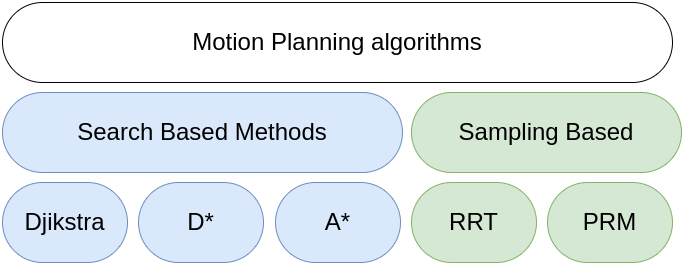
\includegraphics[width=0.7\textwidth]{Images/Background/Trajectory Generation/Motion_planing_algorithms.drawio.png}
    \caption{Scheme of motion planning algorithms~\cite{InesBatista2022Thesis}}
    \label{fig:background:trajectory generation:motion planning algorithms}
\end{figure}

\paragraph{Decomposition based Methods}

Decomposition based algorithms~\cite{latombe2012robot} partition the free configuration space $\mathcal{C}_{\text{free}}$ into a finite number of cells. From this, a connectivity graph $G = (V, E)$ is constructed, where the vertices $V$ represent the cells, and the edges $E$ denote adjacency relationships between the cells. Using this graph, standard graph search algorithms such as Dijkstra’s algorithm~\cite{dijkstra2022note}, $A^{*}$~\cite{hart1968formal}, and $D^{*}$~\cite{stentz1994optimal} can be employed to find a path.

These algorithms guarantee optimally in discrete spaces. However, the computational cost grows quadratically with the size of the search space, making them impractical for high-dimensional or complex environments where computational demands can become prohibitive.

\paragraph{Sampling-Based Methods}

Sampling-based methods~\cite{lavalle2006planning} have gained significant attention in recent years for solving motion planning problems in robotics. These methods rely on randomly sampling the configuration space $\mathcal{C}$ to build feasible paths within $\mathcal{C}_{\text{free}}$. They are generally classified into two subcategories: \textit{multiple-query} methods, which build a reusable graph for solving multiple start-goal pairs $(B, C)$, and \textit{single-query} methods, which focus on solving a single start-goal pair.

\subparagraph{Probabilistic Roadmaps (PRM)} 

PRM~\cite{kavraki1996probabilistic} is a multiple-query algorithm that constructs a roadmap starting from an empty graph $G = (N, E)$. New random configurations, $h_{\text{rand}}$, are added to the set of nodes $N$. If a collision-free path exists between $h_{\text{rand}}$ and its closest neighbors in $N$, edges are added to $E$. This process continues until a termination condition (e.g., time limit or number of configurations) is reached. The resulting graph can then be used with graph-search algorithms to solve various motion planning queries. While PRM enables exploration of large configuration spaces efficiently, it is not complete but probabilistically complete, and the solution quality depends heavily on the number of samples and neighbors considered.

\subparagraph{Rapidly-Exploring Random Trees (RRT)} 

RRT~\cite{lavalle2006planning} is a single-query algorithm that constructs a tree starting from an initial configuration. When a new sample $h_{\text{rand}}$ is generated, the algorithm attempts to connect it to the closest configuration $h_{\text{near}}$ in the tree by generating intermediate configurations ensuring a collision-free path from $h_{\text{near}}$ to $h_{\text{rand}}$. Like PRM, RRT is not complete but probabilistically complete. 

To address this, Bidirectional RRT was developed, where two trees are constructed: one growing from $B$ to $C$ and the other from $C$ to $B$. However, these algorithms are not optimal, meaning the paths found may not be the shortest. To overcome this limitation, RRT* was introduced in~\cite{karaman2011sampling}. In RRT*, new samples are connected to the nearest configuration $h_{\text{near}}$, while ensuring the minimum cost between them. Additionally, the algorithm checks whether $h_{\text{new}}$ provides a better parent-child relationship for neighboring nodes, allowing the tree to be restructured for a lower-cost solution. Though more computationally intensive, RRT* guarantees asymptotic optimality, meaning the path approaches the optimal solution as the number of samples increases.

\paragraph{Artifical potential fields} (APF)~\cite{khatib1985real}, is an approach that uses a potential field to guide the robot towards the goal while avoiding obstacles. To do this, we modelate the goals as being an atractive force, whilest making the obstacles, repulsive force. The sum of forces, the potential, is then the correct direction for the robot to move in. This method is simple and computational efficient, but it can get stuck in local minima, and it there for is not complete, to solve this problem, one can use harmonic potential functions as in \cite{kim1992real,rimon1990exact}.

In table~\ref{tab:path_planning_algorithms}, we summarize the characteristics of the path planning algorithms discussed in this section. Naturally, some algorithms can already be discarded as the computational cost is too high, this means the algorithm we are going to use latter in this work are the RRT and theirs derivations, as well as the APF method


\begin{table}[h]
    \centering
    \caption{Path planning algorithms characteristics.}
    \label{tab:path_planning_algorithms}
    \resizebox{\textwidth}{!}{%
    \begin{tabular}{lcccc}
    \hline
    \textbf{Algorithm}      & \textbf{Completeness} & \textbf{Optimality}       & \textbf{Computational Cost} & \textbf{Approach}       \\ \hline
    Search Based Methods           & complete              & optimal\textsuperscript{1} & high                        & deterministic or heuristic \\
    PRM                     & complete\textsuperscript{2} & non-optimal              & low                         & randomized             \\
    RRT                     & complete\textsuperscript{2} & non-optimal              & low                         & randomized             \\
    RRT*                    & complete\textsuperscript{2} & asymptotic optimal       & low                         & randomized             \\
    APF                     & incomplete            & optimal                   & low                         & deterministic          \\
    \end{tabular}%
    }
    
    \vspace{0.5em}
    \raggedright
    \textsuperscript{1} For discretized space.\\
    \textsuperscript{2} For infinite iterations.
\end{table}
    